%------------------------------------------------------------------------------
% Template file for the submission of papers to IUCr journals in LaTeX2e
% using the iucr document class
% Copyright 1999-2003 International Union of Crystallography
% Version 1.2 (11 December 2002)
%------------------------------------------------------------------------------

\documentclass{iucr}              % DO NOT DELETE THIS LINE

                   %%%%%%%%%%%%%%%%%%%%%%%%%%%%%%%%%%%%%%%%
                   \def\href#1{\relax}\let\foo\caption
%%%%%%%%%%%%%%%%%%%%%%%%%%%%%%%%%%%%%%%%%%%%%%%%%%%%%%%%%%%
% To generate hyperlinked PDF, change the \documentclass line
% to say \documentclass[pdf]{iucr} and process with pdflatex
\ifPDF
  \RequirePackage{hyperref}
  \PassOptionsToPackage{pdftex,bookmarksopen,bookmarksnumbered}{hyperref}
  \voffset=-0.5in
\fi
\let\caption\foo
%%%%%%%%%%%%%%%%%%%%%%%%%%%%%%%%%%%%%%%%%%%%%%%%%%%%%%%%%%%

%------------------------------------------------------------------------------
% Information about the type of paper
%------------------------------------------------------------------------------
     \paperprodcode{a000000}      % Replace with production code if known
     \paperref{xx9999}            % Replace xx9999 with reference code if known
     \papertype{IU}               % Indicate type of article
                                  %   FA - research papers (full article)
                                  %   SC - short communications
                                  %   FC - fast communications
                                  %   LA - lead article
                                  %   TR - topical review
                                  %   XL - crystallization papers
                                  % (Following categories rarely in LaTeX)
                                  %   AA - abstracts
                                  %   AD - addenda and errata
                                  %   AI - inorganic compounds
                                  %   AM - metal-organic compounds
                                  %   AO - organic compounds
                                  %   BC - books received
                                  %   BR - book reviews
                                  %   BI - biography
                                  %   CA - cif applications
                                  %   CD - crystal data
                                  %   CE - current events
                                  %   CI - inorganic compounds
                                  %   CL - calendar of events
                                  %   CM - metal-organic compounds
                                  %   CN - cryocrystallography papers
                                  %   CO - organic compounds
                                  %   CP - computer programs
                                  %   CR - crystallographers
                                  %   CS - scientific comment
                                  %   ED - editorial
                                  %   EI - inorganic compounds
                                  %   EM - metal-organic compounds
                                  %   EO - organic compounds
                                  %   FI - inorganic compounds
                                  %   FM - metal-organic compounds
                                  %   FO - organic compounds
                                  %   IP - issue preface
                                  %   IU - iucr
                                  %   LE - letters to the editor
                                  %   LN - laboratory notes
                                  %   ME - forthcoming meetings/short courses
                                  %   MR - meeting reports
                                  %   NN - notes and news
                                  %   NP - new commercial products
                                  %   OB - obituaries
                                  %   PA - computer program abstracts
                                  %   RI - reference information
                                  %   SG - structural genomics papers
                                  %   SI - short format inorganic compounds
                                  %   SM - short format metal-organic compounds
                                  %   SO - short format organic compounds
                                  %   SP - short structural papers
                                  %   SR - software reviews
                                  %   TE - teaching and education

     \paperlang{english}          % Can be english, french, german or russian
%------------------------------------------------------------------------------
% Information about journal to which submitted
%------------------------------------------------------------------------------
     %\journalcode{A}             % Indicate the journal to which submitted
                                  %   A - Acta Crystallographica Section A
                                  %   B - Acta Crystallographica Section B
                                  %   C - Acta Crystallographica Section C
                                  %   D - Acta Crystallographica Section D
                                  %   J - Journal of Applied Crystallography
                                  %   S - Journal of Synchrotron Radiation
     %-------------------------------------------------------------------------
     % The following entries will be changed as required by editorial staff
     %-------------------------------------------------------------------------
     \journalyr{2003}
     %\journaliss{1}
     %\journalvol{57}
     %\journalfirstpage{1}
     %\journallastpage{11}
     \journalreceived{\relax}
     \journalaccepted{\relax}
     \journalonline{\relax}

\begin{document}                  % DO NOT DELETE THIS LINE

     %-------------------------------------------------------------------------
     % The introductory (header) part of the paper
     %-------------------------------------------------------------------------

     % The title of the paper. Use \shorttitle to indicate an abbreviated title
     % for use in running heads (you will need to uncomment it).

\title{Sample Paper Using the IUCr \LaTeX{} Macro Package\footnote{Version 2}}
\shorttitle{IUCr LaTeX sample}

     % Authors' names and addresses. Use \cauthor for the main (contact) author.
     % Use \author for all other authors. Use \aff for authors' affiliations.
     % Use lower-case letters in square brackets to link authors to their
     % affiliations; if there is only one affiliation address, remove the [a].

     \author[a,b]{J.}{Soape}
     \author[b]{A. N.}{Author}
     \cauthor[a]{John}{Doe}{doe@any.where}{}\aufn{On leave from Institute of
Advanced Research, Albany, Ruritania.}

     \aff[a]{Baskerville Lodge, \city{Dartmoor}, Devon, \country{England}}
     \aff[b]{3 Watery Way, \city{Full Fathom} 5, \country{Atlantis}}

     % Use \shortauthor to indicate an abbreviated author list for use in
     % running heads (you will need to uncomment it).

\shortauthor{Soape, Author and Doe}

     % Use \vita if required to give biographical details (for authors of
     % invited review papers only). Uncomment it.


\vita{Joe Soape is an archetypal generic author, whose association with the
much-travelled Kilroy has extended over many years. He travels to work each
day on a Clapham omnibus.
\\
John Doe is also a generic individual with extensive experience of legal and
forensic matters.}

     % Keywords (required for Journal of Synchrotron Radiation only)
     % Use the \keyword macro for each word or phrase, e.g. 
     % \keyword{X-ray diffraction}\keyword{muscle}

\keyword{\LaTeX}
\keyword{class file}
\keyword{documentation}

     % PDB and NDB reference codes for structures referenced in the article and
     % deposited with the Protein Data Bank and Nucleic Acids Database (Acta
     % Crystallographica Section D). Repeat for each separate structuree.g.
     % \PDBref[dethiobiotin synthetase]{1byi} \NDBref[d(G$_4$CGC$_4$)]{ad0002}

%\PDBreference[optional name]{refcode}
%\NDBreference[optional name]{refcode}

\maketitle                        % DO NOT DELETE THIS LINE

\begin{synopsis}
Documentation of the IUCr \LaTeX{} macro package and a demonstration of its
use in constructing a paper for an IUCr journal.
\end{synopsis}

\begin{abstract}
This document describes how to obtain and use the \emph{iucr} \LaTeX{} macro
package for submitting articles in \LaTeX{}2$\varepsilon$ format to IUCr
journals (\emph{Acta Crystallographica, Journal of Applied Crystallography,
Journal of Synchrotron Radiation}).
\end{abstract}


     %-------------------------------------------------------------------------
     % The main body of the paper
     %-------------------------------------------------------------------------
     % Now enter the text of the document in multiple \section's, \subsection's
     % and \subsubsection's as required.


\section{Purpose}

The International Union of Crystallography (IUCr) publishes a number of
specialist scientific journals, many containing complex mathematics. The
journal articles are held as electronic files for typesetting and electronic
publication. The common format for the article files is SGML, an ISO standard
that allows a specific structure to be defined for a class of documents
through a machine-readable \emph{document type definition} (DTD). Detailed
markup of the article with SGML codes allows portions of the article to be
indexed, hyperlinked or stored in databases. Mathematical formulae within the
document are encoded in \TeX{} \cite{knuth84}, a portable technical
typesetting language.

Authors may submit papers to the IUCr in a variety of electronic formats, some
more suitable than others for automated translation to SGML. A particularly
suitable format is already widespread in many scientific disciplines, namely
a structured dialect of \TeX{} known as \LaTeX{} \cite{lamport86}.

The IUCr has produced a macro package (\emph{iucr}) that may be used by
authors familiar with \LaTeX{} version 2$\varepsilon$ to create articles
that can easily be translated to SGML. This document describes how to use
the package. It has been prepared using the package itself, and refers to some
of its own contents to illustrate relevant points.

Full details of how to obtain the IUCr \LaTeX{} macro package are given in
Appendix~A.

\section{Structure of the paper}

The following skeleton outline indicates the structure of a typical paper in
\LaTeX{} format; portions in parentheses are optional. A file
\textbf{template.ltx} is available by ftp from the IUCr, and includes this
structure with some additional material that is described below. Frequent
reference will be made to this file (it will usually just be called `the
template'). Authors should acquire a copy of the template as the basis of
their journal submission; it is possible, however, to construct a
satisfactory paper from scratch by following the instructions in
this document.

A copy of the template is included as Appendix~D.

\begin{verbatim}
% ------ The front matter (heading section) ---
\documentclass{iucr}
\begin{document}

\title{...}
(\shorttitle{...})

  (\author...)
  \cauthor...
  \aff...

(\shortauthor{...})
(\vita{...})

\maketitle

\begin{synopsis}
...
\end{synopsis}

\begin{abstract}
...
\end{abstract}

% ------ The main body of the text ------------
\section{...}

   Text text text ...

   \subsection{...}

   Text text text ...

      \subsubsection{...}

   Text text text ...

\section{...}

   Text text text ...

% ------ The back matter ----------------------
(\appendix
   \section{...}

   Text text text ...
)

(\ack{...})

\begin{references}
   \reference{...}
\end{references}

\end{document}
\end{verbatim}


\section{Style of the paper}

The same template is used for submitting papers of all types to all the IUCr
journals. Different printing styles are used for different types of papers
and across different journals, and the author should indicate the required
style for the finished paper.

The article \emph{must} begin with a line invoking the IUCr document class;
the minimum required is
%
\begin{verbatim}
\documentclass{iucr}
\end{verbatim}
%
to indicate that \LaTeX{} should load and implement the macros for IUCr journal
articles.

\textbf{The initial submission to a journal Coeditor should use the `preprint'
option} to produce a single-column double-spaced version suitable for examination
and annotation by referees. This may be achieved by modifying the first
statement in the file to
%
\begin{verbatim}
\documentclass[preprint]{iucr}
\end{verbatim}

\textbf{The final version of the paper should then be prepared in the appropriate
style}, and adjustments made to the layout of mathematical equations, tables,
figure widths \emph{etc.} to ensure that such components fit the journals'
multi-column layout.

\emph{Note, however, that the actual page layout of the journals is \textbf{not}
performed using \LaTeX{}; it is therefore not worth spending time trying to
fit the figures and tables into a proper balanced page layout. Except when 
used in the preparation of camera-ready conference proceedings, the different
page styles are used \textbf{only} to allow authors to break equations and 
establish suitable scaling factors for figures.}

If the paper is intended for publication in \emph{Acta Crystallographica
Section A} (\emph{Acta A}) or \emph{Journal of Applied Crystallography}
(\emph{JAC}), the \verb|\documentclass| statement \emph{may} include the
option \verb|a| (in square brackets). If the paper is a
\emph{Short Communication}, the additional option \verb|short| is
\emph{required}.

If the paper is intended for publication in \emph{Acta Crystallographica
Section B} or \emph{Acta Crystallographica Section D} (\emph{Acta B},
\emph{Acta D}), the \verb|\documentclass| statement \emph{must}
include the option \verb|d| (in square brackets). If the paper is a
short contribution, such as a \emph{Short Communication}  or
\emph{Crystallization Paper}, the additional option \verb|short| is required.

If the paper is intended for publication in \emph{Journal of Synchrotron
Radiation} (\emph{JSR}), the \verb|\documentclass| statement \emph{must}
include the option \verb|s| (in square brackets). If the paper is a
\emph{Short Communication}, the additional option \verb|short| is required. 

\medskip
\begin{small}
\begin{tabular}{@{\hskip-1em}l>{\footnotesize}l}%
\emph{Acta A, JAC} full article & \verb|\documentclass{iucr}| \\
\emph{Acta B, D} full article  & \verb|\documentclass[d]{iucr}| \\
\emph{JSR} full article   & \verb|\documentclass[s]{iucr}| \\
\emph{Acta A, JAC} short article & \verb|\documentclass[short]{iucr}| \\
\emph{Acta B, D} short article  & \verb|\documentclass[d,short]{iucr}| \\
\emph{JSR} short article  & \verb|\documentclass[s,short]{iucr}| \\
\end{tabular}
\end{small}

If a paper has been submitted as a camera-ready document for a conference
proceedings issue of the journal, the option \verb|conference| should
be supplied, \emph{e.g.}

\medskip
\begin{small}
\begin{tabular}{@{\hskip-1em}l>{\footnotesize}l}%
\emph{JAC} conference paper & \verb|\documentclass[conference]{iucr}| \\
\emph{JSR} conference paper & \verb|\documentclass[s,conference]{iucr}| \\
\end{tabular}
\end{small}

For such papers, the submission instructions might also request that
authors use the \verb|nohead| option to remove the running headlines
and footers (these will be added by the editorial office during the
subsequent preparation for printing).

A full list of available package options is supplied as Appendix~B.

\penalty-500
\section{The header of the paper}

Information about the paper's title, its authors and their affiliations,
and such descriptive portions of the paper as the \emph{Abstract},
\emph{Synopsis} (which appears as a brief description of the paper in the
Table of Contents of an issue) or \emph{keywords} is included in the
\emph{header} or \emph{front matter} of the paper.

\subsection{The document preamble}

The template contains identifiers that encode bibliographic and production
information about the document. The author may not know all the details
that are required, but should fill in any information that is known, and
leave the remaining default values for IUCr editorial staff to update.

The template includes a complete list of allowed article type codes.

\begin{verbatim}
\paperprodcode{a000000} % Production code
\paperref{xx9999}       % Editorial reference
\papertype{FA}          % Type of article
                        %   FA - Full article
                        %   SC - Short Comm.
\paperlang{english}     % Language
\journalcode{A}         % Which journal?
                        %   A - Acta Cryst. A
                        %   B - Acta Cryst. B
                        %   C - Acta Cryst. C
                        %   D - Acta Cryst. D
                        %   D - Acta Cryst. E
                        %   J - J. Appl. Cryst.
                        %   S - J. Synchr. Rad.
\journalyr{2000}
\journaliss{1}
\journalvol{56}
\journalfirstpage{000}
\journallastpage{000}
\journalreceived{0 XXXXXXX 0000}
\journalaccepted{0 XXXXXXX 0000}
\journalonline{0 XXXXXXX 0000}
\end{verbatim}

The printout of the article's dates of receipt and acceptance and its
online publication date can be suppressed by supplying the argument
\verb|\relax| to the last three commands.

\subsection{The document proper}

The body of the document is introduced with the line
%
\begin{verbatim}
\begin{document}
\end{verbatim}

This must appear \emph{after} the preamble, and \emph{before}
the title or any other content.

\subsection{Title}

Give the title of the paper as an argument to the macro \verb|\title|. The
title will usually be incorporated in a footer to the pages of the
journal. Often the full title is too long to fit within the footer.
If it is necessary to indicate a shorter form of the title for use
in the footer, use the macro \verb|\shorttitle|
%
\begin{verbatim}
\title{Sample Paper Using the IUCr \LaTeX{}
       Macro Package}
\shorttitle{IUCr \LaTeX{} sample}
\end{verbatim}

If a title footnote is required, the \verb|\footnote| macro should be
invoked \emph{inside} the argument to the \verb|\title| macro, \emph{e.g.}
%
\begin{verbatim}
\title{Sample Paper Using the IUCr \LaTeX{}
       Macro Package\footnote{Version 2}}
\end{verbatim}

\subsection{Author group}

The list of the authors' names and addresses forms the \emph{author group}
of the paper. The macros \verb|\cauthor|, \verb|\author| (for names of
correspondence and other authors respectively) and \verb|\aff| (for
\emph{affiliations}) should be used. If the paper has a single author, the
form of the entry will look like this:
%
\begin{verbatim}
\cauthor{J.}{Soape}{soap@bath.tub}{}
\aff{Baskerville Lodge, \city{Dartmoor}, Devon,
     \country{England}}
\end{verbatim}
%
The author's given name(s) or initial(s) appear within the first set
of curly braces, the surname (\emph{i.e.} family name) in the second set.
The third braces give the author's e-mail address, and the fourth the
correspondence address (where this differs from the affiliation printed in
the paper). \textbf{The third and fourth sets of braces must be present,
even if they are empty.}

The associated address is given as the argument to the \verb|\aff| macro.
The country should be indicated by the \verb|\country| macro; the
city of residence \emph{may} (but need not) be indicated by the \verb|\city|
macro. These are both included within the outer set of braces that delimit
the argument of the \verb|\aff| macro.

If there are multiple authors, the simpler \verb|\author| macro is used
for all but the correspondence author. A paper may have only \emph{one}
correspondence author. For example,
%
\begin{verbatim}
\author{J.}{Soape}
\author{A. N.}{Author}
\cauthor{John}{Doe}{doe@any.where}{}

\aff{Baskerville Lodge, \city{Dartmoor}, Devon,
     \country{England}}
\end{verbatim}
%
Where there are multiple addresses, each author should be linked to a
corresponding address by a small letter enclosed in square brackets
immediately following the name of the relevant macro,
%
\begin{verbatim}
\author[a,b]{J.}{Soape}
\author[b]{A. N.}{Author}
\cauthor[a]{John}{Doe}{doe@any.where}{}

\aff[a]{Baskerville Lodge, \city{Dartmoor},
        Devon, \country{England}}
\aff[b]{3 Watery Way, \city{Full Fathom} 5,
        \country{Atlantis}}
\end{verbatim}

Two other macros exist to modify an author's name; these should both appear
\emph{inside} the braces delimiting the surname. They are \verb|\nee| to
describe a married woman's original surname (\emph{e.g.}
\verb|\author{J.}{Jackson \nee{Jones}}|, producing the text `J. Jackson
\nee{Jones}'), and \verb|\jr| to indicate a dynastic relationship.
The macro \verb|\jr| by itself produces the text `Jr'; with an argument
\emph{in square brackets} it produces the text provided, \emph{e.g.}
\verb|\author{H. H.}{Hackenbusch\jr[III]}| produces the
text `H. H. Hackenbusch\jr[III]'.

Footnotes associated with the authors' names \emph{must} use the
\verb|\aufn| macro, which must follow the last mandatory argument of
each occurrence of the
\verb|\author| or \verb|\cauthor| macros:
%
\begin{verbatim}
\cauthor[a]{John}{Doe}{doe@any.where}{}\aufn{On
     leave from Institute of Advanced Research,
     Albany, Ruritania.}
\end{verbatim}

\subsection{Author biography}

Occasionally a biographical note for an author or authors is required
(usually for Lead Articles, Topical Reviews, or other invited contributions).
The \verb|\vita| macro is used to supply the required information;
if there is more than one author, a line containing \verb|\\| should
separate the individual entries:
%
\begin{verbatim}
\vita{Joe Soape is an archetypal generic
      author, whose association with the
      much-travelled Kilroy has extended
      over many years. He travels to work
      each day on a Clapham omnibus.
\\
     John Doe is also a generic individual with
     extensive experience of legal and
     forensic matters.}
\end{verbatim}

\subsection{Other information}

Some journals require other ancillary information to be conveyed in the article
header. These may be supplied at this point in the document.

\emph{Journal of Synchrotron Radiation} requires one or more key words or
phrases for indexing purposes. These may be supplied with the macro
\verb|\keyword|, \emph{e.g.}
%
\begin{verbatim}
\keyword{X-ray diffraction}
\keyword{muscle}
\end{verbatim}

On rare occasions (especially for conference proceedings) an editor may
request that keywords be printed in other journals. In such a case the
document class line should be changed to include the \verb|keywords| option, 
\emph{e.g.}
%
\begin{verbatim}
\documentclass[a,keywords]{iucr}
\end{verbatim}

Conversely, the \verb|nokeywords| option may be used to suppress the output
of the keywords terms in styles where they are printed by default.

\emph{Acta Crystallographica Section D} requires reference codes for structures
deposited in the Protein Data Bank. Use the macros \verb|\PDBref| and
\verb|\NDBref|, \emph{e.g.}
%
\begin{verbatim}
\PDBref[dethiobiotin synthetase]{1byi}
\NDBref[d(G$_4$CGC$_4$)]{ad0002}
\end{verbatim}

\subsection{maketitle}

The command \verb|\maketitle| should be included before the synopsis (or, if
no synopsis is present, before the abstract). This command instructs
\LaTeX{} to output the authors and affiliations in the correct style. If it
is not present, the information will in many cases nevertheless be output
correctly; but several error messages may be generated by \LaTeX{}.


\subsection{Synopsis}

All IUCr journals require the author to provide a brief synopsis of the
paper, a couple of sentences in length, which is printed on the journal
contents pages. There is a \emph{synopsis} environment which should be used
for this purpose:

\begin{verbatim}
\begin{synopsis}
Documentation of the IUCr \LaTeX{} macro
package and a demonstration of its
use in constructing a paper for an
IUCr journal.
\end{synopsis}
\end{verbatim}

By default, the synopsis is printed only for the \verb|preprint| option.
If it is necessary for some reason to display the synopsis within other
styles, the option \verb|synopsis| may be added, \emph{e.g.}

\begin{verbatim}
\documentclass[d,conference,synopsis,nohead]{iucr}
\end{verbatim}
%
will print the synopsis at the end of an unornamented conference-style paper
for \emph{Acta Crystallographica Section D}. When printed, the 
synopsis appears on the \LaTeX{} printout within parallel horizontal
rules at the end of the document.

\subsection{Abstract}

The abstract of the paper should be given in the \emph{abstract}
environment,
%
\begin{verbatim}
\begin{abstract}
This document describes how to obtain and use
the \emph{iucr} \LaTeX{} macro package for
submitting articles in \LaTeX{}2$\varepsilon$
format to IUCr journals (\emph{Acta
Crystallographica, Journal of Applied
Crystallography, Journal of
Synchrotron Radiation}).
\end{abstract}
\end{verbatim}

The abstract must always be a single paragraph. It may \emph{not} contain
footnotes.


\section{The main body of the paper}

The main body of the paper has a relatively simple structure; it consists of
a sequence of sections, which may contain subsections or subsubsections. It
may also include appendices (introduced by the \verb|\appendix| command)
which themselves contain sections or sub- and subsubsections. (Details of
how to mark up appendices are included as Appendix~C.)

The sectional elements of the paper contain the text, broken into paragraphs
that are separated in the \LaTeX{} source by blank lines. The text may
include mathematics (discussed in a separate section below), figures and
tables.

\subsection{A note on single- and double-column formats}

The current template uses the \emph{multicol} package to permit
double-column typesetting in the style of the IUCr journals. The main
purpose of this is to ensure that the author knows where long mathematical
formulae should be broken in order to fit into the journal column widths.

It may occasionally be necessary to switch off double-column setting (or to
restrict it to certain portions of an article that relies heavily on long
mathematical formulae or wide tables that cannot conveniently be fitted into
a single column of the journal).

Within the body of the paper, double-column setting is switched off
by the statement
%
\begin{verbatim}
\onecolumn
\end{verbatim}
%
and may be re-invoked by the declaration
%
\begin{verbatim}
\twocolumn
\end{verbatim}

In short contributions to some sections of \emph{Acta Crystallographica}
three-column setting is used. The macro \verb|\threecolumn| is also
available for switching explicitly to such a mode.

The present version of the \emph{multicol} package does not
permit figures, tables or other `floats' within the multi-column portion of
the article; this is partly the reason why figures and tables should be
inserted at the end of the article (see later).

\subsection{Sectioning}

The text may contain sections nested to a depth of 3, \emph{i.e.} sections,
subsections and subsubsections, introduced respectively by the macros
\verb|\section|, \verb|\subsection| and \verb|\subsubsection|. The title of
the section should follow as an argument to the sectioning command.
\textbf{N.B. Please leave a blank line above and below these commands in the
source file.}
%
\begin{verbatim}
\subsection{Sectioning}

The text may contain sections nested to a depth
of 3, \emph{i.e.} sections, subsections
\end{verbatim}

Please employ the usual \LaTeX{} convention of leaving one or more blank
lines to indicate paragraph breaks. However, displayed equations and
embedded figures should \emph{not} be placed in separate paragraphs. If it is
desired to include some visual white space in the \LaTeX{} source file (and
it can certainly be helpful to lay out complex mathematics neatly and
clearly to permit later editing), lines containing only a \% symbol (the
\LaTeX{} comment code) may be used for visual punctuation, \emph{e.g.}
%
\begin{verbatim}
as seen in the equation
%
\begin{equation}
     x^n + y^n = z^n
\end{equation
%
and discussed elsewhere...
\end{verbatim}

\subsection{Changes of typeface}

Within the body of the text, portions of italic or bold-face type may be
indicated by the \textit{textit} and \textbf{textbf} macros. The material to
be typeset in a different face should be passed as the argument to these
macros, and \emph{not}, as is sometimes done, included within an open macro
declaration inside braces; \emph{i.e.} use
%
\begin{verbatim}
\textbf{bold-face type}
\end{verbatim}
%
and \textbf{not}
%
\begin{verbatim}
{\textbf bold-face type}
\end{verbatim}

However, in keeping with the spirit of \LaTeX{}, it is generally better
style to use the \verb|\emph| macro to highlight text that is to be
emphasised, rather than using specific font commands such as \verb|\textit|.

\subsection{Footnotes}

The use of footnotes in the main body of the paper is discouraged, but
where their use is unavoidable they may normally be handled with the standard
\LaTeX{} \verb|\footnote| macro. This will produce footnotes across the
full width of the page, with automatic numbering.

Exceptionally, however (specifically where camera-ready documents are to
be prepared strictly in the style of the journals), manual placement of
footnotes is possible\fnmark{}.

The macro \verb|\fnmark| is used to indicate the location in the text of
the current footnote marker. Footnotes are numbered in sequence through an
article. If it is necessary to over-ride the automatic number generation,
an optional argument (in square brackets) may be supplied. The
\verb|\fnmark| macro does not print a space after the footnote marker, so
when used in the body of a sentence will often be followed by an empty
pair of braces to ensure that a space is printed,

\begin{verbatim}
The use of a footnote marker\fname{} causes a
superscript numeral to be printed; the numbers
are auto-incremented. Very occasionally\fname[3],
a specific number needs to be given in square
brackets. 
\end{verbatim}

The actual text of the footnotes is given as an argument to the
\verb|\fntext| macro. Although the footnote numbers are automatically
tracked by the \verb|\fnmark| macro, the number associated with
each footnote \emph{must} be given in square brackets as the first
argument to the \verb|\fntext| macro. If the number is omitted, the
footnote will be printed without a number.

The user must collect together footnotes handled in this way at the relevant
location in the text so that they will be 
printed at the foot of the
first or second column, as required. The macro \verb|\footnotes|,
immediately preceding the first \verb|\fntext| macro of a group, will
print the separator rule (horizontal line).

It is the responsibility of the user to ensure that paragraphs that
need to be broken to allow placement of the footnotes are correctly
formatted. An example of how to do this with the \verb|\breakpar| and
\verb|\noindent| commands is shown in the example.

\footnotes
\fntext[2]{The default placement of footnotes across the full page width
is a shortcoming of the way in which floats are handled by the
\emph{multicol} package. Use of the macros described here allows manual
placement in either column.}

\noindent
\begin{verbatim}
... may be necessary to break a paragraph
\breakpar

\footnotes
\fntext[1]{Note the use of empty braces after a call
           to the fnmark macro to ensure that a
           space is printed.}
\fntext[3]{When the normal numbering is overridden
           by the use of an optional argument to
           fnmark, one must remember to change the
           footnote text numbering accordingly.}

\noindent
to allow placement of the footnotes. 
\end{verbatim}


\section{Mathematics}

The standard \LaTeX{} conventions for typesetting mathematics should be
employed. In-line equations are delimited by the \verb|\(| and \verb|\)|
constructs, so that an equation embedded within running text such as
\verb|\(x^n+y^n=z^n\)| would print as \(x^n+y^n=z^n\). Displayed equations
without numbering are obtained with the \verb|\[| and \verb|\]| constructs,
\emph{e.g.}
\begin{verbatim}
\[ x = -b \pm \frac{\sqrt{b^2-4ac}}{2a} \]
\end{verbatim}
%
displays as
%
\[
  x = -b \pm \frac{\sqrt{b^2-4ac}}{2a}
\]

Numbered display equations are obtained with the \emph{equation}
environment,
%
\begin{verbatim}
\begin{equation}
x = -b \pm \frac{\sqrt{b^2-4ac}}{2a}
\end{equation}
\end{verbatim}
%
yielding
%
\begin{equation}
  x = -b \pm \frac{\sqrt{b^2-4ac}}{2a}
\end{equation}

\section{Acknowledgements and references}

\subsection{Acknowledgements}

The acknowledgements should appear in a single paragraph as argument to the
\verb|\ack| macro:
%
\begin{verbatim}
\ack{The assistance and knowledge of \TeX{},
     \LaTeX{} and SGML of many members of the
     IUCr editorial staff are acknowledged.}
\end{verbatim}

\subsection{References}

Reference lists may be built up in two ways: manually, or with the
assistance of the Bib\TeX{} program and associated bibliographic database
files.

\subsubsection{Plain citations}

If bibliographic references are being handled manually, they should be cited
in the text using the Harvard system which employs the surname of the author
and year of publication. Parenthetic allusions (Parth\'e \& Gelato, 1984)
may be made by including the authors' names and the date of publication
within parentheses; direct textual references normally have the date in
parentheses, as in this reference to the work of \citeasnoun{rauch76}.

The reference list is then built up by establishing a \emph{references}
environment, and placing each cited work within a \verb|\reference| entry:
%
\begin{verbatim}
\begin{references}
\reference{Parth\'e, E. \& Gelato, L. (1984).
   \emph{Acta Cryst.} A\textbf{40}, 169--183.}
\reference{Rauch, H. \& Petrascheck, D. (1976).
   \emph{Grundlagen f\"ur ein
   Laue-Neutroneninterferometer Teil 1:
   Dynamische Beugung.} Report AIAU 74405b.
   Atominstitut der \"Osterreichischen
   Universit\"aten, Austria.}
\end{references}
\end{verbatim}

\subsubsection{Using Bib\TeX{}}

The Bib\TeX{} program package may be used to handle citations and reference
lists, such as to the seminal work of \citeasnoun{pauling89}
and other multi-author articles \cite{pargel84}. The IUCr bibliography
style file \textbf{iucr.bst} should be obtained and loaded in a public
directory to obtain correctly-formatted reference lists and citations.

In this case the in-text citation is handled by the normal Bib\TeX{}
conventions. Note in the following listing the use of the commands
\verb|\citeasnoun| and \verb|\cite| to obtain citations that occur as
part of the running text or as parenthetic insertions respectively.
%
\begin{verbatim}
The Bib\TeX{} program package may be used to
handle citations and reference lists, such
as to the seminal work of \citeasnoun{pauling89}
and other multi-author articles \cite{pargel84}.
\end{verbatim}

The references section is invoked by placing the declaration
%
\begin{verbatim}
\referencelist[foo,bar]
\end{verbatim}
%
just before the \verb|\end{document}| statement. The \verb|\referencelist|
command takes a list of names of bibliographic databases as its argument in
square brackets (in this example, the references would be found in either of
the files \textbf{foo.bib} or \textbf{bar.bib} in the author's filesystem).
\textbf{Any such bibliographic database files must accompany the submission.}
If the \verb|\referencelist| command is given without any argument, the
bibliographic information is expected to be in a file called
\textbf{iucr.bib}. Generation and formatting of the reference list itself
is handled by Bib\TeX{}.

See Lamport \citeyear{lamport86} for further information about Bib\TeX{}. An
example of a sequence of \LaTeX{}/Bib\TeX{} runs necessary to generate the
final version of this document is given in Appendix~A.
\goodbreak
\section{Floating objects (tables and figures)}

As mentioned previously, floats such as tables and figures are not handled
properly within the double-column environment provided by the
\emph{multicol} package; they are also not yet automatically handled by the
page make-up software in use at the Editorial offices. Therefore, tables
and figures are best placed \emph{after} the rest of the document.

An exception is made for papers solicited as camera-ready conference
proceedings. In these cases, the author should manually place tables and
figures within the text at the top or bottom of columns where possible; or
between paragraphs if unavoidable.

\subsection{Tables}

Several \LaTeX{} styles exist for tables (because they are complicated
objects that exist in a variety of styles). It is likely that the table
translator will pose the greatest number of problems. Currently we recommend
authors to use the \emph{tabular} style for simple tables. Other table
packages, such as \emph{supertabular} or \emph{longtable} may be used for
complex tables at the author's discretion.

Authors should, however, be aware that it might be counterproductive for
them to expend too much effort in producing \LaTeX{} tables that are visually
attractive, since at a detailed level they may conflict with the layout
requirements of the SGML version of the tables that will ultimately be produced.

\subsubsection{Simple tables using the \emph{tabular} style}

Table 1 shows a simple table set using the following code:
%
\begin{verbatim}
\begin{table}
\caption{Example table}
\begin{tabular}{llccrc}
     & Triplets &       &       & +ve  quartets
                                         &       \\
$E_3$& no.      & \%    & $E_4$ & no.    & \%    \\
\hline
6.0  &   21     & 100   & 6.0   &    185 & 100   \\
4.0  &  143     & 100   & 4.0   &   1213 & 100   \\
3.0  &  353     & 100   & 3.0   &   3295 & 100   \\
2.5  &  583     &  99.8 & 2.5   &   5813 &  99.8 \\
2.0  &  980     &  99.7 & 2.0   & 10,006 &  99.5 \\
1.5  & 1823     &  99.2 & 1.5   & 13,114 &  98.8 \\
1.0  & 3395     &  96.9 &       &        &       \\
\end{tabular}
\end{table}
\end{verbatim}
%
In this example, the \verb|{llccrc}| argument instructs the \verb|tabular|
environment to align material within the six tables of the columns against
the left margin (\verb|l|), centred (\verb|c|), or aginst the right margin
(\verb|r|) of each table cell.

\medskip
\begin{table}
\caption{Example table}
\begin{tabular}{llccrc}
     & Triplets
            &       &       & +ve  quartets
                                      &      \\
$E_3$& no.  & \%    & $E_4$ & no.    & \%    \\
\hline
6.0  &   21 & 100   & 6.0   &    185 & 100   \\
4.0  &  143 & 100   & 4.0   &   1213 & 100   \\
3.0  &  353 & 100   & 3.0   &   3295 & 100   \\
2.5  &  583 &  99.8 & 2.5   &   5813 &  99.8 \\
2.0  &  980 &  99.7 & 2.0   & 10,006 &  99.5 \\
1.5  & 1823 &  99.2 & 1.5   & 13,114 &  98.8 \\
1.0  & 3395 &  96.9 &       &        &       \\
\end{tabular}
\end{table}

\subsection{Figures}

Figures may be included using the following segment of code as an example:
%
\begin{verbatim}
\begin{figure}
\caption{Example of PostScript figure.}
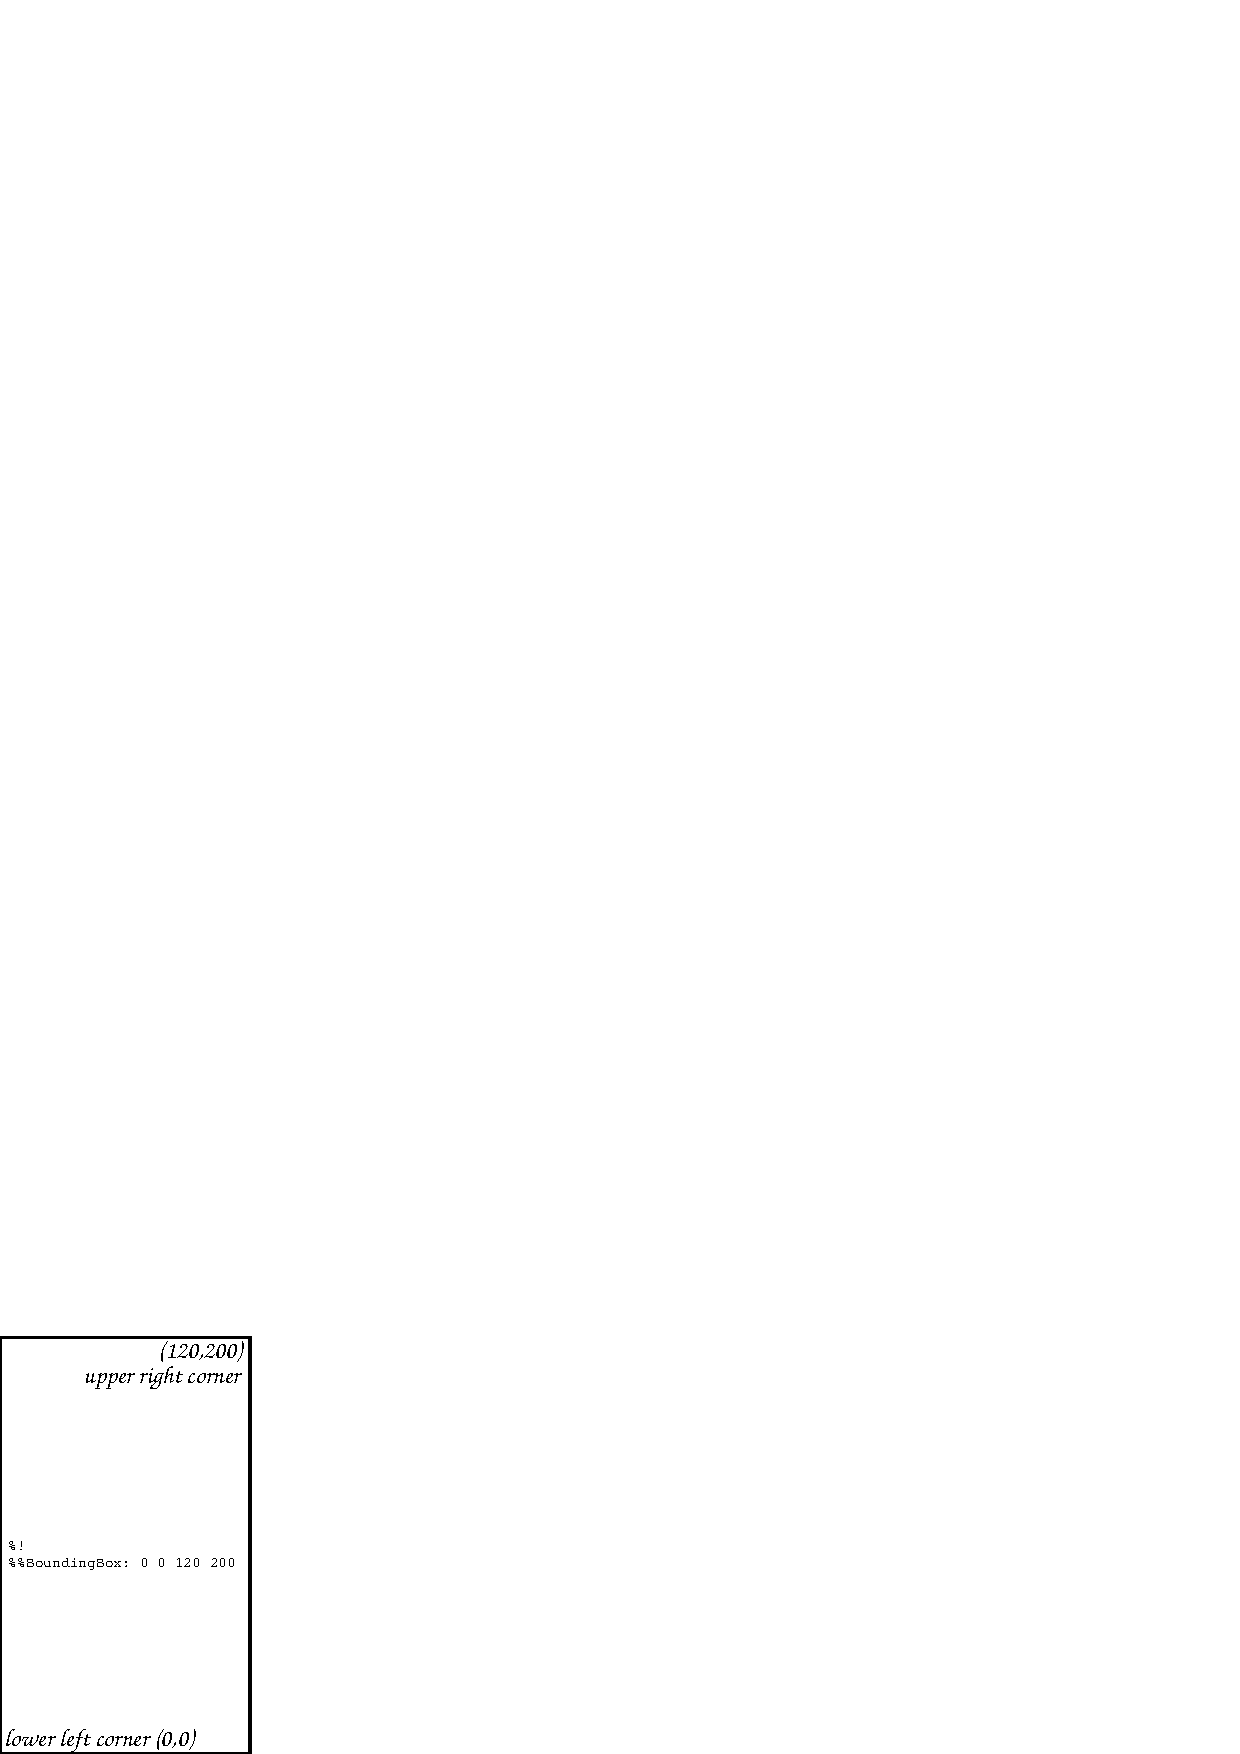
\includegraphics{fig1}
\end{figure}
\end{verbatim}
If no file extension is supplied, then the graphics driver routines
available through \LaTeX{} graphics packages (usually \emph{dvips} or
\emph{pdflatex}) will search the current directory for files beginning with
the name supplied and with extension suitable for the supported
graphics file formats (\textit{e.g.} .eps, .ps for \emph{dvips}, .png,
.jpg, .pdf for \emph{pdflatex}).
%
If figures in a supported format are not available, each figure caption should
nevertheless be supplied in the form above. (That is, set up a \emph{figure}
environment around each \verb|\caption| entry.)

If the space that will be occupied by a figure is known, it is possible to
reserve that space in the document by creating a dummy PostScript file that
indicates the \emph{bounding box} of the figure. Fig.1 indicates the
reference points at the lower-left and upper-right corners of a rectangular
box that is said to \emph{bound} the figure. The $x, y$ coordinates of these
reference points (measured in \emph{points} or units of
\(\textstyle\frac{1}{72}\) of an inch) are specified in a PostScript
\verb|%%BoundingBox| directive. In other words, if the PostScript figure
reproduced here as Fig.~1 were unavailable, a file fig1.ps containing the
two lines
%
\begin{verbatim}
%!
%%BoundingBox: 0 0 120 200
\end{verbatim}
%
could be constructed to reserve the appropriate space for later insertion of
the figure (the line containing \verb|%!| is an obligatory header for
PostScript files).

If it is necessary to scale a figure to fit into the available space, the
command \verb|\scalebox| may be used as in this example (to scale by 80\%):

\begin{figure}
\caption{Example of PostScript figure.}
\ifPDF
  %\hskip.5in\pdfximage{fig1.pdf}
  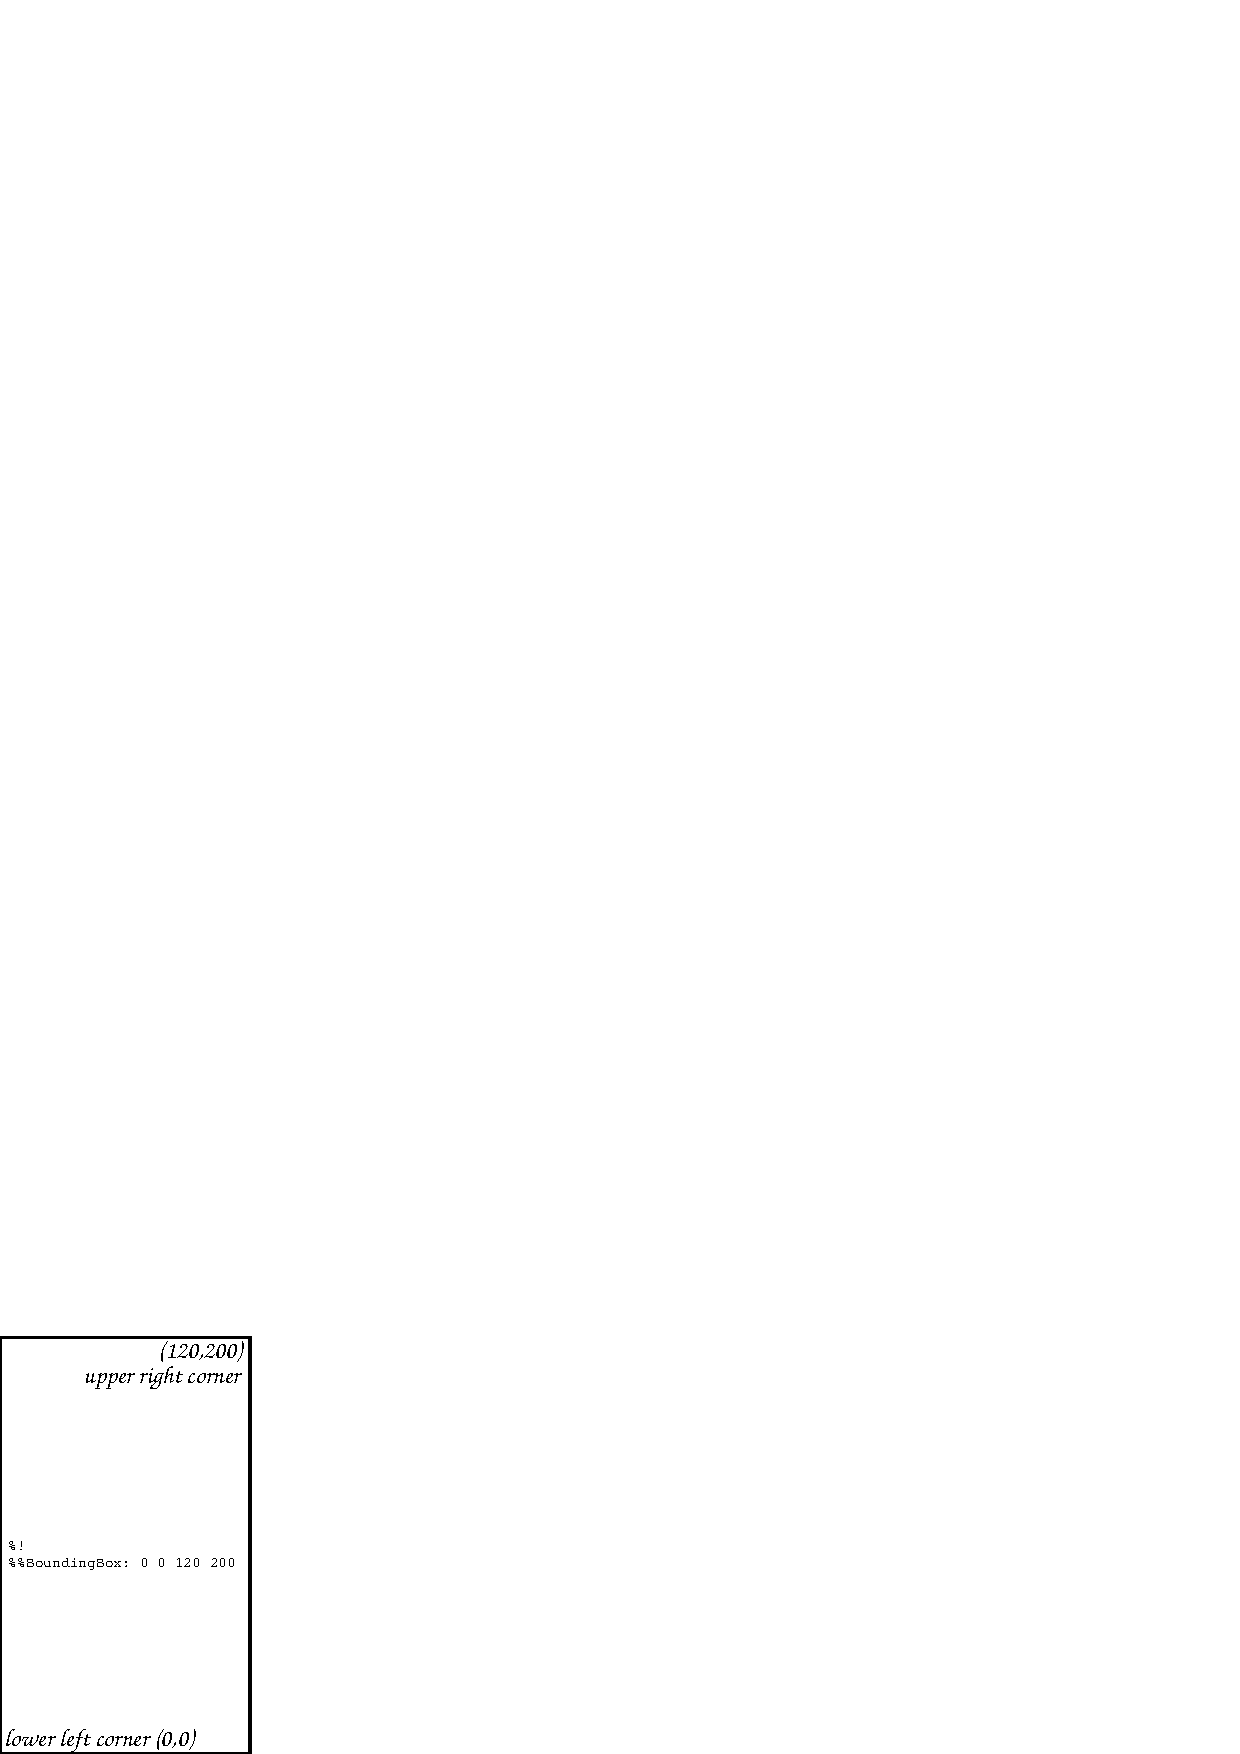
\includegraphics{fig1.pdf}
\else
  \includegraphics{fig1.ps}
\fi
\end{figure}
%
\begin{verbatim}
\scalebox{.8}{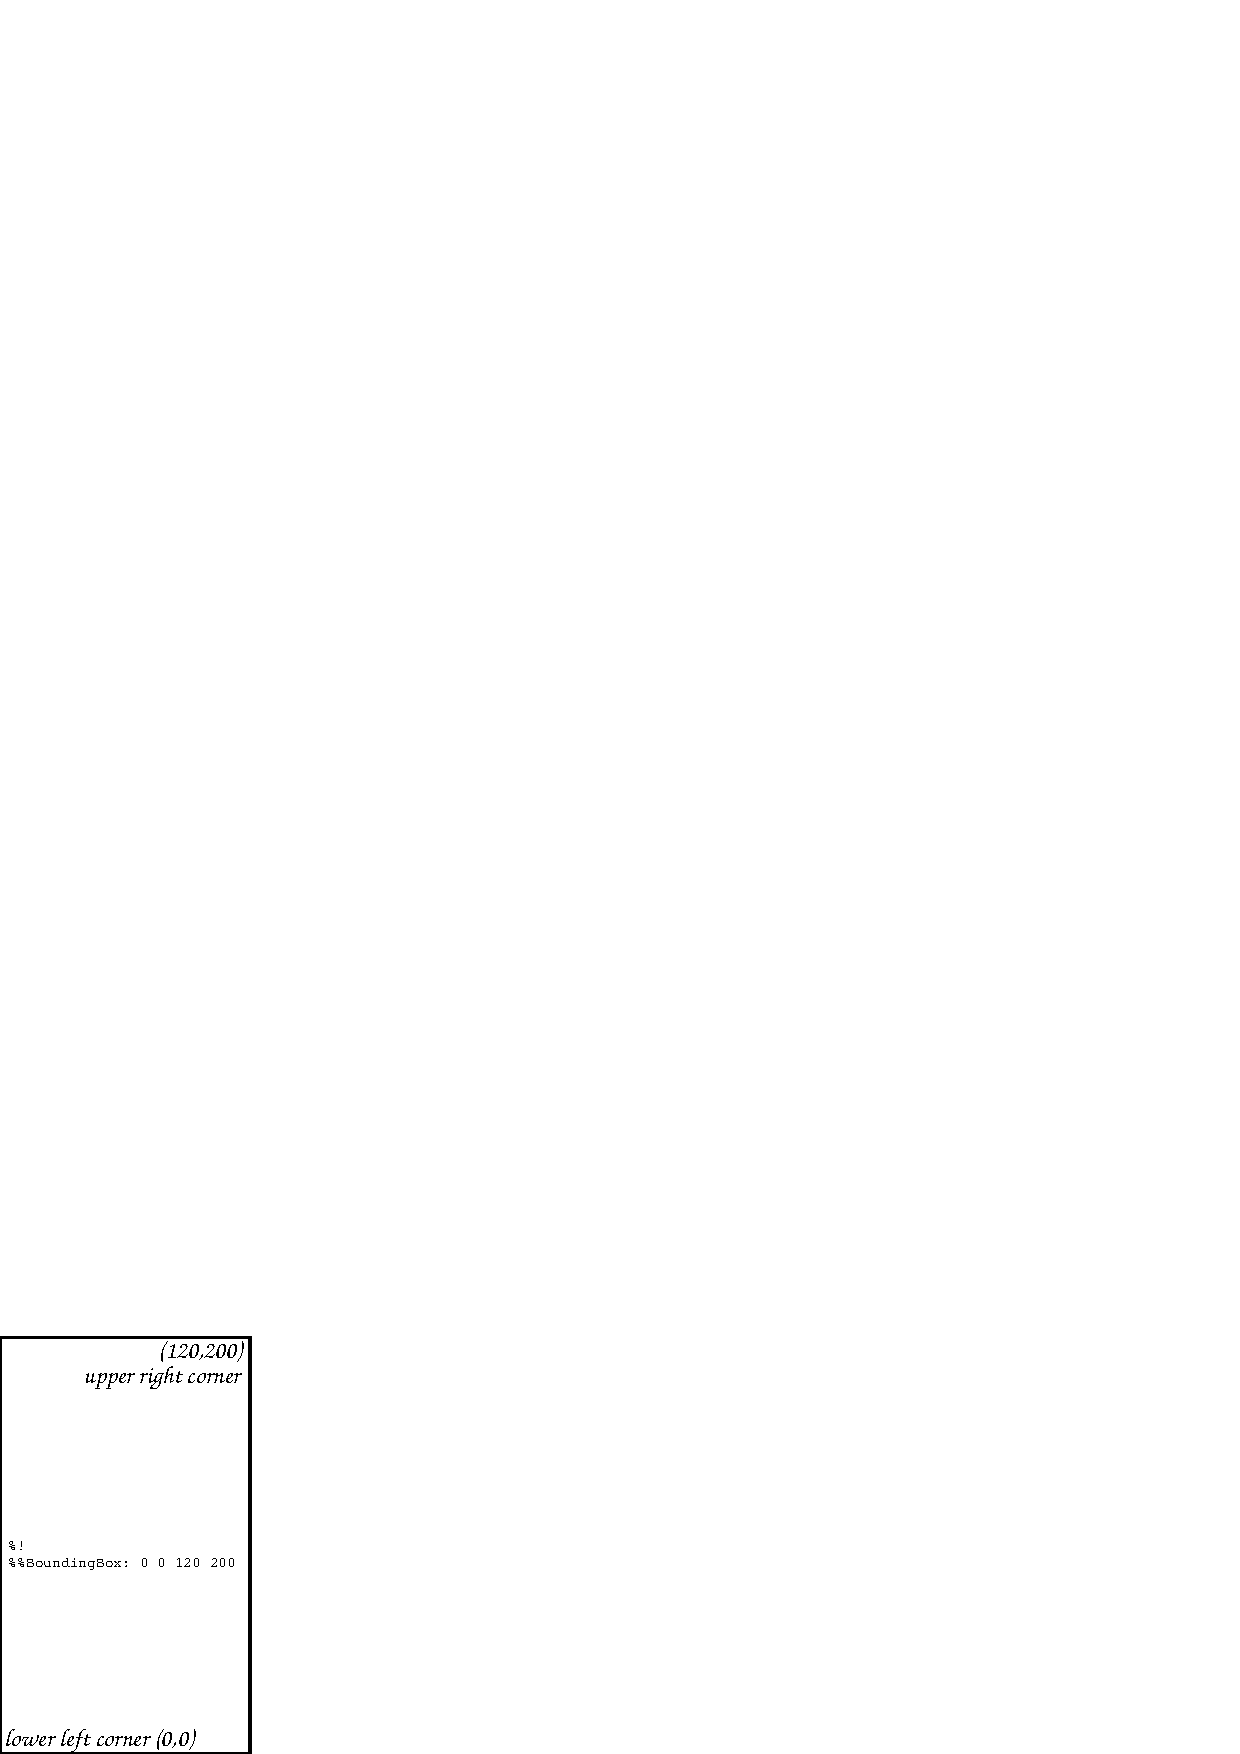
\includegraphics{fig1}}
\end{verbatim}
%
Note how the \verb|\includegraphics| command is enclosed in braces.


\subsubsection{Advanced handling of graphics}

The handling of figures described above depends on the
availability of the \LaTeX{} \emph{graphics} package. More sophisticated
graphics handling is possible if the \emph{graphicx} package is available.
To use \emph{graphicx} in place of \emph{graphics}, the following line
should be added to the preamble of the document, just after the
\verb|\documentclass{iucr}| line:
%
\begin{verbatim}
\RequirePackage{graphicx}
\end{verbatim}
% 
Then rotation of a figure through a right angle (for example) could be
accomplished with the command
%
\begin{verbatim}
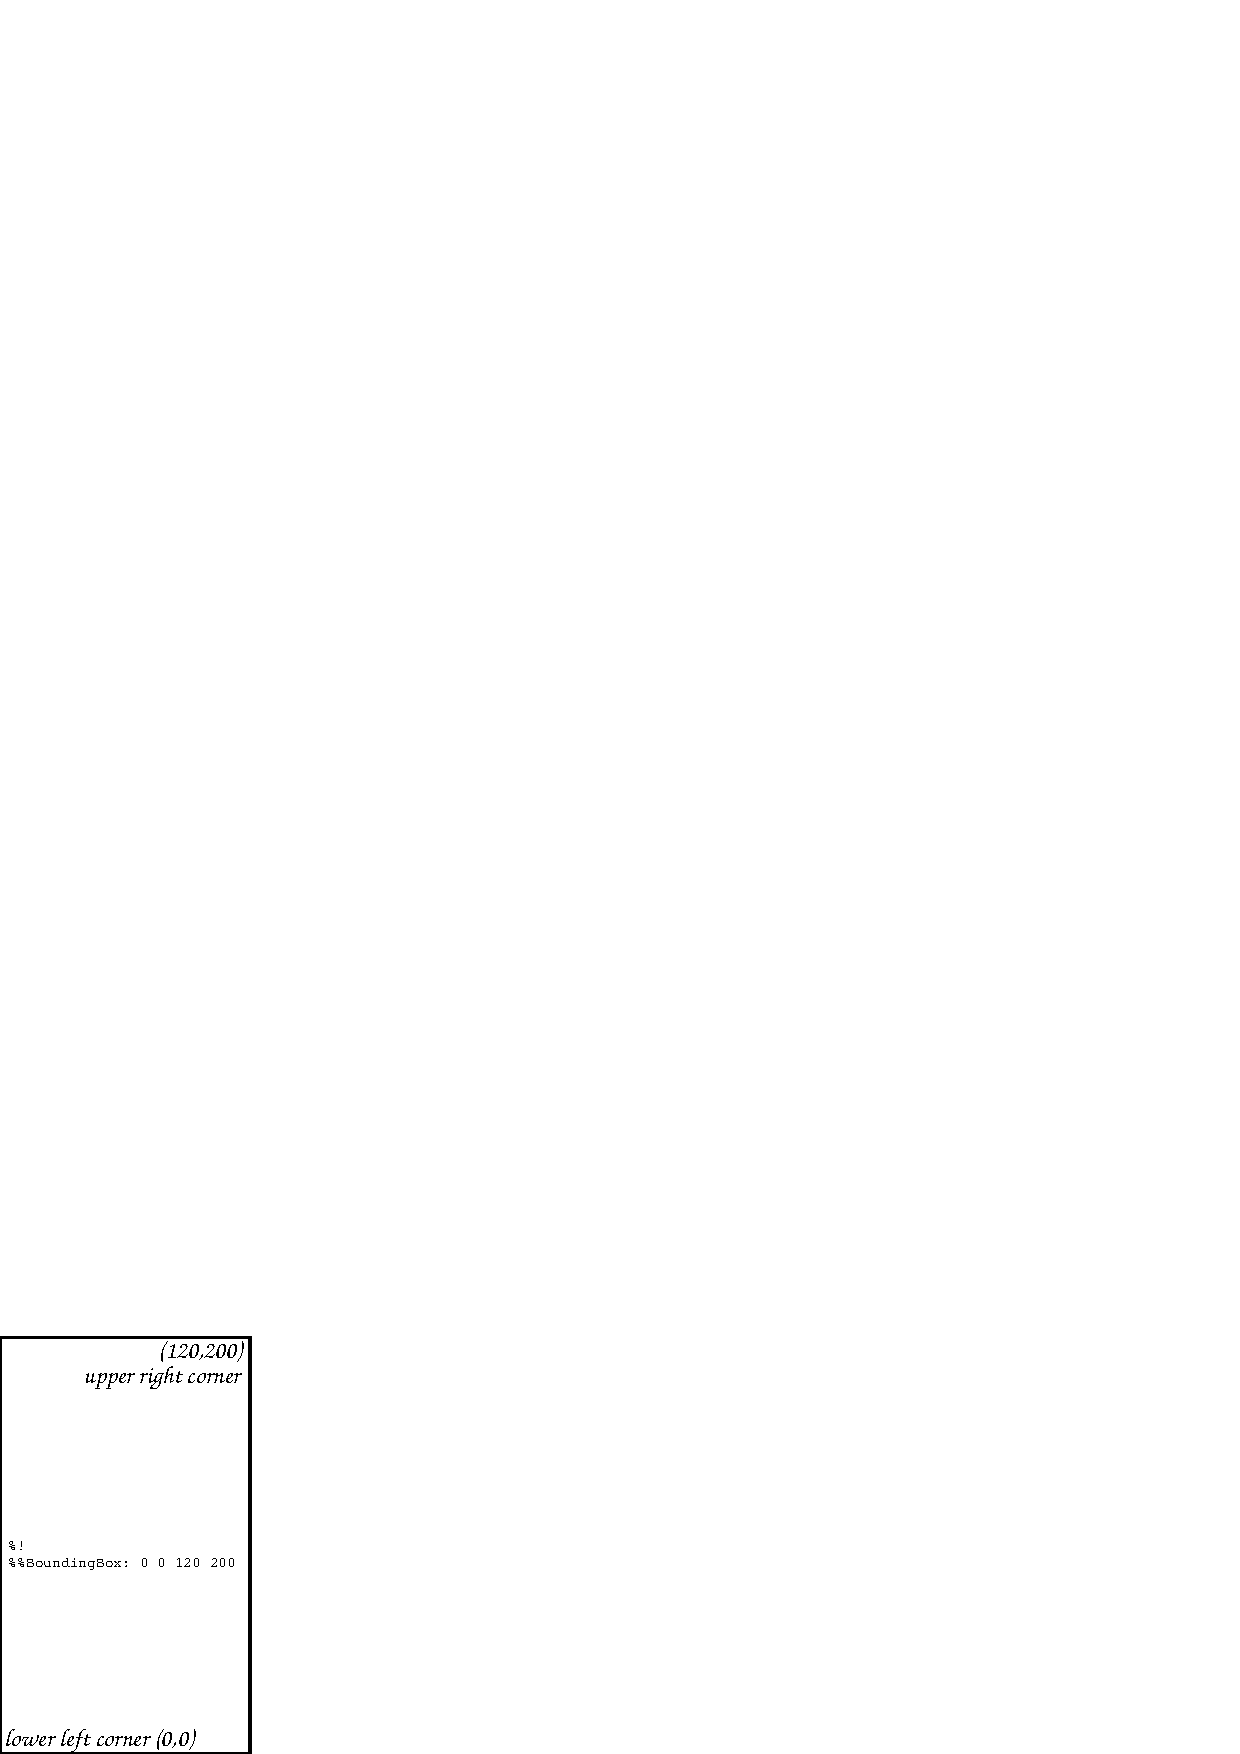
\includegraphics[angle=90]{fig1}
\end{verbatim}
%
See local documentation of the \emph{graphicx} package for further
information.

\section{Conference abstracts}

From time to time the IUCr publishes abstracts of Conference proceedings
as supplements to its journals. A conference abstract may be submitted in a 
suitable format by using the \verb'abstract' option to the
\verb'\documentclass' statement, \textit{i.e.}

\begin{verbatim}
\documentclass[abstract]{iucr}
\end{verbatim}

For a conference abstract, only the following components are required: a
title (using the \verb'\title' macro); the author names and affiliations as 
described in Section~4.4; keywords
(Section~4.6 -- note that for Conference abstracts the
\verb'keyword' option is \emph{not} required in the \verb'\documentclass'
line); the body of the abstract within an \textit{abstract} environment;
and a reference list constructed as plain citations
(Section~7.2.1). For Conference abstracts \emph{only},
references should be indicated by numbers in square brackets, [1], [2],
\textit{etc.}, in the text. Numbering is generated automatically within the 
reference list.

Figures and tables may also be used sparingly in Conference abstracts. They 
are treated in the same way as other document types, and should be
positioned at the appropriate locations within the body of the abstract.

A distinct template for Conference abstracts is available as the file
\textbf{abstemplate.ltx} (see Appendix~A for availability). A sample
Conference abstract is included as Appendix~E.



\section{Miscellaneous notes}

\subsection{Changed font encoding}

A \LaTeX{} warning similar to the following may appear when modes other
than the \emph{preprint} mode are used:

\begin{verbatim}
LaTeX Font Warning: Encoding `OML' has changed to 
(Font)              `OT1' for symbol font `letters'
                    in the math version `bold' on
                    input line 485.
\end{verbatim}
%
This is harmless (indicating some internal font manipulations) and may be
ignored.

\subsection{Fonts unavailable}

The journal styles use the \LaTeX{} new font selection scheme and attempt
to use PostScript fonts in the Times, Helvetica and Palatino families where
available. These are accessible to many \LaTeX{} distributions. If they
are not available, however, the \emph{preprint} mode should nonetheless
function satisfactorily using only the Computer Modern fonts that come as
standard with the great majority of \TeX{} distributions.

Some authors may find that they have Times PostScript fonts available, but
not Palatino, which is used in several of the article styles. In this case
they may add the \verb|nopalatino| option to their \verb|\documentclass|
declaration.

Authors with access to Optima PostScript fonts may use the \verb|optima| 
option with the \verb|\documentclass| declaration to produce a result
identical to that obtained in the editorial/production office. For 
copyright reasons, these fonts are not freely distributable.

\subsection{Underfull and overfull boxes}

\LaTeX{} will report underfull and overfull boxes (corresponding to text
which does not properly fill the contents of a line or page). While these
messages can indicate real problems and should be investigated, it must be
remembered that the journal pages will not be typeset using \LaTeX{}, and it
is therefore a waste of time to try to eliminate all such warnings.

\subsection{Direct creation of PDF}

The option \verb|pdf| in the documentclass invocation will allow the file
to be processed by the pdf\LaTeX{} command where available, so producing
an output file in Adobe Portable Document Format (PDF). In such a case, the
author should include figures in PDF rather than PostScript format. Details
of the pdf\LaTeX{} package are available from
\href{http://tug.org/applications/pdftex}{http://tug.org/applications/pdftex}.


\subsection{Improvements to the class file}

Reports of bugs and suggestions for improvements to the class file are
welcome, and should be addressed to Brian McMahon at the IUCr (bm@iucr.org).

     % Appendices appear after the main body of the text. They are prefixed by
     % a single \appendix declaration, and are then structured just like the
     % body text.


\appendix
\section{Obtaining the IUCr \LaTeX{} package}

The \LaTeX{} package may be obtained by anonymous ftp from the IUCr server
\textbf{ftp.iucr.org}. Login as user \emph{anonymous} and supply your email
address as password. Change to the templates/latex directory. Transfer in
text mode the following files (only the first two are essential for the
use of the package):

\href{ftp://ftp.iucr.org/templates/latex/iucr.cls}{\textbf{iucr.cls}},
the class file containing all the macros detailed in this document;

\href{ftp://ftp.iucr.org/templates/latex/template.ltx}{\textbf{template.ltx}},
the skeleton template file used to construct a submission;

\href{ftp://ftp.iucr.org/templates/latex/abstemplate.ltx}{\textbf{abstemplate.ltx}},
the template file used for Conference abstracts \emph{only};

\href{ftp://ftp.iucr.org/templates/latex/documentation.ltx}%
{\textbf{documentation.ltx}}, this document;

\href{ftp://ftp.iucr.org/templates/latex/fig1.ps}{\textbf{fig1.ps}},
the PostScript figure included in this document as an example;

\href{ftp://ftp.iucr.org/templates/latex/iucr.bib}{\textbf{iucr.bib}},
a Bib\TeX{} bibliography file for this document;

\href{ftp://ftp.iucr.org/templates/latex/iucr.bst}{\textbf{iucr.bst}},
the IUCr Bib\TeX{} style file.

Test your ability to run \LaTeX{} on this file. A \emph{complete} processing
run will involve three passes of the \LaTeX{} program and one of Bib\TeX{}; on
a typical Unix workstation, the processing run will usually require the
commands
%
\begin{verbatim}
% latex documentation.ltx
% bibtex documentation
% latex documentation.ltx
% latex documentation.ltx
\end{verbatim}

If successful you should be able to preview the documentation on screen
(\emph{e.g.} with the Unix \emph{xdvi} program) or print it (\emph{e.g.}
with Unix \emph{dvips}).

If the tests are successful, the package file \textbf{iucr.cls} should be
installed in a public class directory (the location of which will be system
dependent) or copied into any directory containing files which are processed
with the \emph{iucr} package.

\subsection{Compatibility}

The \emph{iucr} package has been designed for \LaTeX{}2$\varepsilon$ and
will only work with that format. The development version of \LaTeX{}
was 
\begin{small}\verb|LaTeX2e <1998/12/01> patch level 1|\end{small}
as distributed on the \TeX{} User Group \TeX{}Live4 CD-ROM (see
\href{http://www.tug.org/texlive/}{http://www.tug.org/texlive/}
for details).

\subsection{Ancillary packages}

The \emph{iucr} macros also use a number of public packages that are
distributed with \LaTeX{} (\emph{e.g. nfss, multicol, dvips, float, harvard,
tabularx}). If these are not available on your system, they may be found in
the \textbf{utilities} subdirectory of the ftp directory indicated above. If
a required package is not available at your site or in the
\textbf{templates/latex/utilities} subdirectory, please send an email to
\textbf{bm@iucr.org} for assistance.


\goodbreak

\section{Complete list of package options}

The table below summarises the options available to modify the behaviour
of the \emph{iucr} package. All those relevant to the current journal
article styles have been discussed in the body of the current article.

In general, one may select a single page style and concatenate other
options in a comma-separated list. Where mutually exclusive options
are listed, precedence is assigned based on the order of definitions
within the class file, and so is not predictable.

The \emph{vanilla} style provides a two-column style with typography
similar to that used in \emph{Acta Crystallographica} but without a number 
of the journal-specific features. The \emph{it} style is for use by
authors of chapters of \emph{International Tables for Crystallography}.
The \emph{o} and \emph{x} styles recreate an earlier page layout of the
journals and are retained purely for historical interest.

\begin{table}[2]
\caption{One or more of the options listed below may be added in square
brackets to the declaration of the document class.}
\begin{tabular}{ll}
\textit{Journal styles} \\
%\hline
  (no options)      & \textit{Acta A}/\textit{JAC} full article (default) \\
  \verb|a|          & \textit{Acta A}/\textit{JAC}                 \\
  \verb|c|          & \textit{Acta C}                              \\
  \verb|d|          & \textit{Acta B}/\textit{Acta D}              \\
  \verb|e|          & \textit{Acta E}                              \\
  \verb|s|          & \textit{JSR}                                 \\
\hline
\textit{Article styles} \\
%\hline
  \verb|full|       & full article (default)   \\
  \verb|short|      & short communication      \\
  \verb|conference| & conference paper         \\
\hline
\textit{Other styles} \\
%\hline
  \verb|preprint|   & preprint (1 col., wide-spaced)      \\
  \verb|it|         & International Tables chapter        \\
  \verb|abstract|   & Conference abstracts                \\
  \verb|vanilla|    & vanilla (general) style             \\
  \verb|o|          & old \textit{Acta A}/\textit{JAC}    \\
  \verb|x|          & old  \textit{JSR}                   \\
\hline
\textit{Special directives} \\
%\hline
  \verb|nohead|     & do not print page header/footer      \\
  \verb|keywords|   & print keywords (default for \textit{JSR} and
  conference abstracts) \\
  \verb|nosynopsis| & do not print keywords                \\
  \verb|synopsis|   & print synopsis (default in preprint) \\
  \verb|nosynopsis| & do not print synopsis                \\
  \verb|pdf|        & allow processing with pdflatex       \\
\hline
\textit{Font selections} \\
%\hline
  \verb|optima|     & use Optima fonts                     \\
  \verb|nopalatino| & do not use Palatino fonts            \\
\end{tabular}
\end{table}

\goodbreak

\section{Marking up appendices}

\subsection{Placement}

Appendices are regarded in the IUCr DTD as an integral part of the
\emph{body matter} of the paper, unlike in many other DTDs, including the
ISO 12083 standard for scientific articles, where they are deemed to be part
of the \emph{back matter}. This means that they are inserted \emph{before}
the acknowledgements section.

\subsection{Invocation}

The appendices form the last portion of the body matter, and are introduced
by a single declaration of the form
%
\begin{verbatim}
\appendix
\end{verbatim}
%
Thereafter, each appendix should be considered as a new section, and may
contain subsections and subsubsections, following the same structure as the
main body of the text. Appendix headings are generated automatically,
\emph{e.g.}
%
\begin{verbatim}
\appendix
\section{Marking up appendices}

\subsection{Placement}

Appendices are regarded in the IUCr DTD...
\end{verbatim}

\onecolumn

\section{The template.ltx template file}

Below is given a complete listing of the template file \textbf{template.ltx}.
The article that you are now reading was constructed using version 1.2 of
the template, and you may find it useful to examine its source code (it is
available as the file \textbf{documentation.ltx} in the IUCr macro distribution
package).


\begin{verbatim}
%------------------------------------------------------------------------------
% Template file for the submission of papers to IUCr journals in LaTeX2e
% using the iucr document class
% Copyright 1999-2003 International Union of Crystallography
% Version 1.2 (11 December 2002)
%------------------------------------------------------------------------------

\documentclass{iucr}              % DO NOT DELETE THIS LINE

     %-------------------------------------------------------------------------
     % Information about the type of paper
     %-------------------------------------------------------------------------
     \paperprodcode{a000000}      % Replace with production code if known
     \paperref{xx9999}            % Replace xx9999 with reference code if known
     \papertype{FA}               % Indicate type of article
                                  %   FA - research papers (full article)
                                  %   SC - short communications
                                  %   FC - fast communications
                                  %   LA - lead article
                                  %   TR - topical review
                                  %   XL - crystallization papers
                                  % (Following categories rarely in LaTeX)
                                  %   AA - abstracts
                                  %   AD - addenda and errata
                                  %   AI - inorganic compounds
                                  %   AM - metal-organic compounds
                                  %   AO - organic compounds
                                  %   BC - books received
                                  %   BR - book reviews
                                  %   BI - biography
                                  %   CA - cif applications
                                  %   CD - crystal data
                                  %   CE - current events
                                  %   CI - inorganic compounds
                                  %   CL - calendar of events
                                  %   CM - metal-organic compounds
                                  %   CN - cryocrystallography papers
                                  %   CO - organic compounds
                                  %   CP - computer programs
                                  %   CR - crystallographers
                                  %   CS - scientific comment
                                  %   ED - editorial
                                  %   EI - inorganic compounds
                                  %   EM - metal-organic compounds
                                  %   EO - organic compounds
                                  %   FI - inorganic compounds
                                  %   FM - metal-organic compounds
                                  %   FO - organic compounds
                                  %   IP - issue preface
                                  %   IU - iucr
                                  %   LE - letters to the editor
                                  %   LN - laboratory notes
                                  %   ME - forthcoming meetings/short courses
                                  %   MR - meeting reports
                                  %   NN - notes and news
                                  %   NP - new commercial products
                                  %   OB - obituaries
                                  %   PA - computer program abstracts
                                  %   RI - reference information
                                  %   SG - structural genomics papers
                                  %   SI - short format inorganic compounds
                                  %   SM - short format metal-organic compounds
                                  %   SO - short format organic compounds
                                  %   SP - short structural papers
                                  %   SR - software reviews
                                  %   TE - teaching and education

     \paperlang{english}          % Can be english, french, german or russian
     %-------------------------------------------------------------------------
     % Information about journal to which submitted
     %-------------------------------------------------------------------------
     \journalcode{A}              % Indicate the journal to which submitted
                                  %   A - Acta Crystallographica Section A
                                  %   B - Acta Crystallographica Section B
                                  %   C - Acta Crystallographica Section C
                                  %   D - Acta Crystallographica Section D
                                  %   E - Acta Crystallographica Section E
                                  %   J - Journal of Applied Crystallography
                                  %   S - Journal of Synchrotron Radiation
          %--------------------------------------------------------------------
          % The following entries will be changed as required by editorial staff
          %--------------------------------------------------------------------
     \journalyr{2003}
     \journaliss{1}
     \journalvol{59}
     \journalfirstpage{000}
     \journallastpage{000}
     \journalreceived{0 XXXXXXX 0000}
     \journalaccepted{0 XXXXXXX 0000}
     \journalonline{0 XXXXXXX 0000}

\begin{document}                  % DO NOT DELETE THIS LINE

     %-------------------------------------------------------------------------
     % The introductory (header) part of the paper
     %-------------------------------------------------------------------------

     % The title of the paper. Use \shorttitle to indicate an abbreviated title
     % for use in running heads (you will need to uncomment it).

\title{Title of Paper}
%\shorttitle{Short Title}

     % Authors' names and addresses. Use \cauthor for the main (contact) author.
     % Use \author for all other authors. Use \aff for authors' affiliations.
     % Use lower-case letters in square brackets to link authors to their
     % affiliations; if there is only one affiliation address, remove the [a].

\cauthor[a]{Forename}{Surname}{email}{address if different from \aff}
\author[b]{Forename}{Surname}

\aff[a]{First affiliation address \country{England}}
\aff[b]{Second affiliation address}

     % Use \shortauthor to indicate an abbreviated author list for use in
     % running heads (you will need to uncomment it).

%\shortauthor{Soape, Author and Doe}

     % Use \vita if required to give biographical details (for authors of
     % invited review papers only). Uncomment it.

%\vita{Author's biography}

     % Keywords (required for Journal of Synchrotron Radiation only)
     % Use the \keyword macro for each word or phrase, e.g. 
     % \keyword{X-ray diffraction}\keyword{muscle}

%\keyword{keyword}

     % PDB and NDB reference codes for structures referenced in the article and
     % deposited with the Protein Data Bank and Nucleic Acids Database (Acta
     % Crystallographica Section D). Repeat for each separate structure e.g
     % \PDBref[dethiobiotin synthetase]{1byi} \NDBref[d(G$_4$CGC$_4$)]{ad0002}

%\PDBref[optional name]{refcode}
%\NDBref[optional name]{refcode}

\maketitle                        % DO NOT DELETE THIS LINE

\begin{synopsis}
Supply a synopsis of the paper for inclusion in the Table of Contents.
\end{synopsis}

\begin{abstract}
Abstract goes here.
\end{abstract}


     %-------------------------------------------------------------------------
     % The main body of the paper
     %-------------------------------------------------------------------------
     % Now enter the text of the document in multiple \section's, \subsection's
     % and \subsubsection's as required.

\section{Section title}

Text text text text text text text text text text text text text text
text text text text text text text.

\subsection{Title}

Text text text text text text text text text text text text text text
text text text text text text text.

\subsubsection{Title}

Text text text text text text text text text text text text text text
text text text text text text text.


     % Appendices appear after the main body of the text. They are prefixed by
     % a single \appendix declaration, and are then structured just like the
     % body text.

\appendix
\section{Appendix title}

Text text text text text text text text text text text text text text
text text text text text text text.

\subsection{Title}

Text text text text text text text text text text text text text text
text text text text text text text.

\subsubsection{Title}

Text text text text text text text text text text text text text text
text text text text text text text.


     %-------------------------------------------------------------------------
     % The back matter of the paper - acknowledgements and references
     %-------------------------------------------------------------------------

     % Acknowledgements come after the appendices

\ack{Acknowledgements}

     % References are at the end of the document, between \begin{references}
     % and \end{references} tags. Each reference is in a \reference entry.

\begin{references}
\reference{Author, A. \& Author, B. (1984). \emph{Journal} \textbf{Vol}, 
first page--last page.}
\end{references}

     %-------------------------------------------------------------------------
     % TABLES AND FIGURES SHOULD BE INSERTED AFTER THE MAIN BODY OF THE TEXT
     %-------------------------------------------------------------------------

     % Simple tables should use the tabular environment according to this
     % model

\begin{table}
\caption{Caption to table}
\begin{tabular}{llcr}      % Alignment for each cell: l=left, c=center, r=right
 HEADING    & FOR        & EACH       & COLUMN     \\
\hline
 entry      & entry      & entry      & entry      \\
 entry      & entry      & entry      & entry      \\
 entry      & entry      & entry      & entry      \\
\end{tabular}
\end{table}

     % Postscript figures can be included with multiple figure blocks

\begin{figure}
\caption{Caption describing figure.}
\includegraphics{fig1.ps}
\end{figure}

\end{document}                    % DO NOT DELETE THIS LINE
%%%%%%%%%%%%%%%%%%%%%%%%%%%%%%%%%%%%%%%%%%%%%%%%%%%%%%%%%%%%%%%%%%%%%%%%%%%%%%
\end{verbatim}

%\twocolumn

\section{Example of a Conference abstract}

The example below demonstrates how a short Conference abstract may be
presented using the \verb'abstract' option in the \verb'\documentclass'
specification. Such abstracts are normally requested for camera-ready
preparation of Conference proceedings volumes such as those produced for
IUCr Congresses and other large international meetings.

%\onecolumn

\begin{verbatim}
%------------------------------------------------------------------------------
% Template file for the submission of conference abstracts to IUCr journals
% in LaTeX2e using the iucr document class (iucr.cls version 2.0beta 13
% dated 2003/11/24 or later)
% Copyright 2003 International Union of Crystallography
% Version 1.0 (24 December 2003)
%------------------------------------------------------------------------------

\documentclass[abstract]{iucr}              % DO NOT DELETE THIS LINE

\begin{document}                  % DO NOT DELETE THIS LINE

     %-------------------------------------------------------------------------
     % The introductory (header) part of the abstract
     %-------------------------------------------------------------------------

     % The title of the abstract.

\title{Example conference abstract}

     % Authors' names and addresses. Use \cauthor for the main (contact) author.
     % Use \author for all other authors. Use \aff for authors' affiliations.
     % Use lower-case letters in square brackets to link authors to their
     % affiliations; if there is only one affiliation address, remove the [a].

\cauthor{Brian}{McMahon}{bm@iucr.org}{}

\aff{IUCr, 5 Abbey Square, Chester CH1 2HU, \country{UK}}

     % Keywords. Use the \keyword macro for each word or phrase, e.g. 
     % \keyword{X-ray diffraction}\keyword{muscle}

\keyword{\LaTeX}
\keyword{example}
\keyword{conference abstract style}

\maketitle                        % DO NOT DELETE THIS LINE

     %-------------------------------------------------------------------------
     % The main body of the abstract
     %-------------------------------------------------------------------------
\begin{abstract}
This is an example of a conference abstract, such as might be supplied to
an IUCr Congress[1]. It uses a subset of the macros and commands of the
\textit{iucr} macro class, as documented in the class user guide[2]. The
entire text of the abstract should be confined to a single column of
printed text, and preferably should be presented as a single paragraph of
text. References are indicated by bracketed numbers in the text; the
numbering in the reference list is autogenerated, and so the author must
take care to match the numbering correctly. Although discouraged, figures
and tables may be embedded within the abstract text where essential; for
brevity they are omitted from this example, but templates are provided in
the abstemplate.ltx file[3].
\end{abstract}

     %-------------------------------------------------------------------------
     % The back matter of the abstract - references
     %-------------------------------------------------------------------------
     % References are at the end of the document, between \begin{references}
     % and \end{references} tags. Each reference is in a \reference entry.

\begin{references}
\reference{International Union of Crystallography (2002). Abstracts of the
XIX IUCr Congress, Geneva, Switzerland, 6--15 August 2002. \textit{Acta Cryst.}
A\textbf{58} Suppl.}
\reference{International Union of Crystallography (2003). \textit{Sample
Paper Using the IUCr \LaTeX{} Macro Package}.
http://www.iucr.org/iucr-top/journals/latex/documentation.pdf}
\reference{International Union of Crystallography (2003). Template file for 
  Conference abstracts using the iucr.cls \LaTeX{} style.
ftp://ftp.iucr.org/templates/latex/abstemplate.ltx}
\end{references}

\end{document}                    % DO NOT DELETE THIS LINE
%%%%%%%%%%%%%%%%%%%%%%%%%%%%%%%%%%%%%%%%%%%%%%%%%%%%%%%%%%%%%%%%%%%%%%%%%%%%%%
\end{verbatim}

\twocolumn

\ack{The assistance and knowledge of \TeX{}, \LaTeX{} and SGML of many
members of the IUCr editorial staff are acknowledged. Thanks are due to Bruce
Ravel, Julie Cross, Matt Newville, Klas Andersson, Phil Bentley, Loic
Bertrand, Gunnar Thorkildsen, Chris Cousins, Thomas Proffen, Christian
Anders Cumbaa and other users who provided valuable feedback during the
development of the macros and associated templates.}


\begin{references}

\noindent\emph{\scriptsize{(This block generated from the \emph{references}
environment, the other by  Bib\TeX{}.)}}

\reference{Parth\'e, E. \& Gelato, L. (1984). \emph{Acta Cryst.} A\textbf{40},
169--183.}
\reference{Rauch, H. \& Petrascheck, D. (1976). \emph{Grundlagen f\"ur ein
Laue-Neutroneninterferometer Teil 1: Dynamische Beugung.} Report AIAU
74405b. Atominstitut der \"Osterreichischen Universit\"aten, Austria.}

\end{references}

% \referencelist
\bibliographystyle{iucr}
\bibliography{iucr} 



     %-------------------------------------------------------------------------
     % TABLES AND FIGURES SHOULD BE INSERTED AFTER THE MAIN BODY OF THE TEXT
     %-------------------------------------------------------------------------

     % Simple tables should use the tabular environment according to this
     % model


     % Postscript figures can be included with multiple figure blocks


\end{document}
